\section{Feeding relations, factorisation and components}\label{sec:feeding}
\begin{definition}[feeding digraph, blocks]\label{def:feeding}
For labels $A\ne B$ say that $A$ \emph{feeds} $B$ if $\gcd(A+1,B)>1$ (a prime of $A+1$ divides $B$: running $A$ produces a resource that $B$ consumes). The \emph{feeding digraph} of a multiset $C$ has the distinct labels of $C$ as vertices and the pairs $(A,B)$ with $A$ feeding $B$ as edges. Its strongly connected components are the \emph{blocks}; the condensation is acyclic, so the blocks can be listed in a \emph{topological order}, feeders first: if $A$ feeds $B$ then the block of $A$ is not later than the block of $B$.
\end{definition}
\begin{lemma}[NF: non-feeding pairs commute]\label{lem:NF}
If $x$ does not feed $y$ and $(x,y)$ is admissible from a state $s$, then $(y,x)$ is admissible from $s$. Consequently, for $x\neq y$ with $x$ not feeding $y$, an adjacent pair $(x,y)$ in an admissible word can always be exchanged to $(y,x)$.
\end{lemma}
\begin{proof}
$\gcd(x+1,y)=1$ gives $\gcd(y,(x+1)^2)=1$, so $K((x,y))=xy$ by \cref{prop:diamond}(a). Also $K((y,x))=xy/\gcd(x,(y+1)^2)$ divides $xy$. Hence $K((y,x))\mid K((x,y))\mid s$.
\end{proof}
\prov{CW-0350}{NF}{PROVED}{FULL}
\begin{theorem}[block factorisation]\label{thm:F2}
Let $C$ be a multiset (repeated labels allowed) with blocks $B_1,\dots,B_r$ in topological order, $C_i$ the sub-multiset of $C$ on $B_i$, and $m_0=m$, $m_i=m_{i-1}R(C_i)$. Then
\[
 \nu(C,m)=\prod_{i=1}^r\nu(C_i,m_{i-1}),
\]
where $\nu(C_i,y)$ is read as $0$ if $y$ is not an integer. In particular $\nu(C,m)=0$ as soon as one factor is $0$.
\end{theorem}
\begin{proof}
\emph{Sorting.} Let $w$ be admissible from $m$ and let $x,y$ be adjacent letters of $w$ with $x$ in a later block than $y$. Then $x$ does not feed $y$ (an edge $x\to y$ would put the block of $x$ no later than that of $y$), so by \cref{lem:NF} exchanging them is a legal swap. A stable bubble sort by block index reaches the block-sorted word $u_1\cdots u_r$, where $u_i$ is the subword of $w$ on $C_i$, by legal swaps of letters of different blocks; so $u_1\cdots u_r$ is admissible, hence each $u_i$ is admissible from $m_{i-1}$ (the state after $u_1\cdots u_{i-1}$ is $m_{i-1}$ whatever the orders inside the $u_j$).
\emph{Invariant.} Let $\pi_i(w)$ be the subword of $w$ on $C_i$. A legal swap of two letters from different blocks leaves every $\pi_i$ unchanged. A legal swap of two letters of the same block $B_i$ changes only $\pi_i$, by one exchange of adjacent distinct letters (the letters are adjacent in $w$, hence in $\pi_i$); sorting $w$ and the swapped word gives two admissible block-sorted words that differ by this exchange inside the $i$-th segment, so the exchange is a legal swap in $\mathrm{Sw}(C_i,m_{i-1})$. Therefore the tuple of classes $([\pi_1(w)],\dots,[\pi_r(w)])$ is constant on swap classes of $C$ at $m$.
\emph{Bijection.} The map $w\mapsto([\pi_i(w)])_i$ from swap classes to $\prod_i\{\text{classes of }\mathrm{Sw}(C_i,m_{i-1})\}$ is onto: concatenating admissible block words $v_i$ from $m_{i-1}$ gives an admissible word, because the entry state of block $i$ is $m_{i-1}$ whatever was chosen before. It is injective: two words with the same tuple are connected by sorting both and then moving inside each block along a path of $\mathrm{Sw}(C_i,m_{i-1})$; each such step is a legal swap of the whole word, since the state before block $i$ is $m_{i-1}$ in both.
\end{proof}
\prov{CW-0351}{F2}{PROVED}{FULL}
\begin{corollary}[acyclic feeding digraph]\label{cor:F1}
If every block is a single label (the feeding digraph is acyclic), then $\nu(C,m)\le1$ for every $m$. Moreover for the block-sorted word $\tau$ one has $K(\tau)\mid K(w)$ for every arrangement $w$, so $K(\tau)$ is the universal minimal threshold, and $\mathcal A(m)$ is a lower set of the weak order determined by $\tau$ (\cref{sec:feasible}).
\end{corollary}
\begin{proof}
Each $C_i$ is a power of one letter and has one arrangement, so each factor of \cref{thm:F2} is $0$ or $1$. For the second claim, a legal exchange of an inverted pair (relative to $\tau$) turns an admissible word $w$ into an admissible $w'$ (\cref{lem:NF}); applying it at the source $m=K(w)$ shows $K(w')\mid K(w)$, and bubble sort ends at $\tau$.
\end{proof}
\prov{CW-0351}{F2}{PROVED}{FULL}
\begin{remark}
An acyclic feeding digraph is a \emph{sufficient} condition for connectivity at every source; it is not necessary (a strongly connected content may never split; see \cref{ex:sccnever}). Conversely, a split needs a block with at least $3$ labels: a block with at most two distinct labels, each once, has at most two arrangements, which are adjacent, so for contents of distinct labels such a block never splits.
\end{remark}

\subsection{Hub descent}
\begin{proposition}[hub-descent criterion]\label{prop:hub}
Call an arrangement $h$ of $C$ a \emph{hub} if $K(h)\mid K(w)$ for all arrangements $w$ and every $w$ has a path $w=v_0,v_1,\dots,v_s=h$ in $\mathcal G(C)$ with $K(v_{i+1})\mid K(v_i)$. If a hub exists then $\nu(C,m)\le1$ for all $m$.
\end{proposition}
\begin{proof}
If $w\in\mathcal A(m)$ then $K(h)\mid K(w)\mid m$ and every $v_i$ on the descent path has $K(v_i)\mid K(w)\mid m$, so $w$ is joined to $h$ inside $\mathrm{Sw}(C,m)$.
\end{proof}
\prov{CW-0352}{Hub-descent}{PROVED}{FULL}
The criterion is sufficient but not necessary. \emph{Finite-exact census:} over the $4060$ contents of three distinct labels in $\{1,\dots,30\}$, $3408$ have a hub and never split, none has a hub and a split, $525$ have neither a hub nor a split, and $127$ split (all without a hub); for four distinct labels in $\{1,\dots,14\}$ the counts are $773/0/125/103$.
\prov{CW-0353}{CONNECTIVITY:Census-on-three-labels-FINITE}{FINITE-EXACT}{FINITE}

\subsection{Three distinct labels}
For a multiset $S$ of labels, $\kappa(S)$ is as in \cref{sec:threshold}. For three distinct labels the arrangement graph is the hexagon.
\begin{theorem}[exact classification of three distinct labels]\label{thm:T3}
Let $C=\{x,y,z\}$ consist of three distinct labels. The swap graph of $C$ at $m$ is disconnected if and only if there is a labelling $(a,b,c)$ of $C$ such that
\[
 a\mid m,\quad c\mid m,\quad \kappa\{a,b\}\mid m,\quad \kappa\{b,c\}\mid m,\quad \kappa\{a,b,c\}\mid m,\qquad b\nmid m,\quad \kappa\{a,c\}\nmid m .
\]
In that case $\mathcal A(m)=\{(a,b,c),(c,b,a)\}$, an antipodal pair of the hexagon, and $\nu(C,m)=2$. A content has a split source iff for some labelling $L=\lcm(a,c,\kappa\{a,b\},\kappa\{b,c\},\kappa\{a,b,c\})$ is divisible by neither $b$ nor $\kappa\{a,c\}$; the split sources of that labelling are the multiples $m$ of $L$ with $b\nmid m$ and $\kappa\{a,c\}\nmid m$.
\end{theorem}
\begin{proof}
($\Leftarrow$) By \cref{cor:P} the prefix multisets of $(a,b,c)$ are $\{a\},\{a,b\},C$ and of $(c,b,a)$ are $\{c\},\{c,b\},C$, all feasible by hypothesis ($\kappa\{a\}=a$, $\kappa\{c\}=c$). The words $(a,c,b)$ and $(c,a,b)$ have the prefix multiset $\{a,c\}$ and $(b,a,c)$, $(b,c,a)$ have $\{b\}$; both are infeasible by hypothesis ($\kappa\{b\}=b$). So $\mathcal A(m)$ is the antipodal pair, which is disconnected.
($\Rightarrow$) Let $\mathcal A(m)$ be disconnected and $u,w$ in different components. If $u,w$ were at distance $2$ in the hexagon, their unique common neighbour $v$ arises from $u$ and from $w$ by exchanges at different positions, so each prefix multiset of $v$ is a prefix multiset of $u$ or of $w$; by \cref{cor:P} $K(v)\mid\lcm(K(u),K(w))\mid m$, so $v\in\mathcal A(m)$ and $u,w$ would be connected. Hence any two vertices in different components are antipodal. A vertex has a unique antipode, so no component contains two vertices (they would both be antipodal to every vertex of another component) and there are at most two components. Thus $\mathcal A(m)=\{w,w^{\mathrm{rev}}\}$; write $w=(a,b,c)$. Its prefix multisets $\{a\},\{a,b\},\{c\},\{c,b\},C$ are feasible, which gives the five divisibilities; the four other arrangements are inadmissible, and $(a,c,b)$ (resp.\ $(b,a,c)$) has $\{a,c\}$ (resp.\ $\{b\}$) as its only prefix multiset not among the feasible ones, so $\kappa\{a,c\}\nmid m$ and $b\nmid m$. The last statements follow by taking the least $m$ satisfying the divisibilities.
\end{proof}
\prov{CW-0354}{T3}{PROVED}{FULL}
\begin{remark}
The mechanism in words: $b$ alone is infeasible (it consumes something that only $a$ or $c$ produces) and $\{a,c\}$ together is infeasible (they consume something only $b$ produces); everything else is feasible. The two histories can only be run ``through $b$'' from the ends and cannot be exchanged into each other.
\end{remark}

\subsection{The family \texorpdfstring{$\{2,3,N\}$}{{2,3,N}}}
\begin{theorem}[the family $\{2,3,N\}$]\label{thm:23N}
Let $N\ge4$, $N\ne2,3$, and $C=\{2,3,N\}$.
\begin{enumerate}[label=(\alph*),itemsep=1pt]
\item The feeding digraph of $C$ is strongly connected iff $N\equiv2$ or $3\pmod 6$ (then $N\ge8$). Otherwise its blocks are $\{2,3\}$ and $\{N\}$ and $\nu(C,m)\le1$ for every $m$.
\item If $N\equiv2,3\pmod6$ then $\nu(C,m)=2$ iff $m=Nt$ with $\gcd(t,6)=1$, and $\nu(C,m)\le1$ otherwise. In particular $C$ has a split source iff $N\equiv2,3\pmod6$, and then the minimal split source is $N$ itself, where $\mathcal A(N)$ is $\{(2,3,N),(N,3,2)\}$ for $N\equiv2$ and $\{(N,2,3),(3,2,N)\}$ for $N\equiv3\pmod 6$.
\end{enumerate}
\end{theorem}
\begin{proof}
(a) $2$ and $3$ feed each other ($\gcd(3,3)=3$, $\gcd(4,2)=2$). $N$ feeds $2$ iff $N$ is odd; $N$ feeds $3$ iff $3\mid N+1$; $2$ feeds $N$ iff $3\mid N$; $3$ feeds $N$ iff $N$ is even. So $N$ lies in the block of $\{2,3\}$ iff ($N$ odd or $N\equiv2\bmod3$) and ($N$ even or $3\mid N$), which is $N\equiv2,3\pmod 6$ by inspecting the six residues. Otherwise the blocks $\{2,3\}$ and $\{N\}$ each have at most one arrangement up to an adjacent exchange, so every factor of \cref{thm:F2} is $\le1$.
(b) Let $N\equiv2\pmod 6$: $N$ is even, $3\nmid N$, $3\mid N+1$; write $a=v_2(N)\ge1$, $N=2^aR$ with $R$ odd and prime to $3$, and $c=v_3(N+1)\ge1$. Direct computation of $\Delta$ gives $\kappa\{2\}=2$, $\kappa\{3\}=3$, $\kappa\{N\}=N$, $\kappa\{2,3\}=1$ (as $R(2)R(3)=24$), $\kappa\{2,N\}=2^{a+1}R=2N$, $\kappa\{3,N\}=2^{\max(0,a-4)}R$ and $\kappa\{2,3,N\}=2^{\max(0,a-3)}R$ (for the primes $q\ge5$ only the consumption $v_q(N)$ matters, and $3$ is produced by $2$, $N$ and consumed only by $3$). By \cref{cor:P}, $K(2,3,N)=2^{\max(1,a-3)}R$ and $K(N,3,2)=N$ both divide $N$, while $K(2,N,3)$, $K(N,2,3)$ are multiples of $2N$ and $K(3,\cdot,\cdot)$ of $3$, none of which divides $N$. So $\mathcal A(N)=\{(2,3,N),(N,3,2)\}$, antipodal, $\nu(C,N)=2$. For general $m$ use \cref{thm:T3}: the middle label $b$ must not divide $m$ while the two ends do. If $b=2$ then $2\nmid m$, but $N$ is an end, so $2\mid N\mid m$, a contradiction. If $b=N$ then one of $\kappa\{a,b\},\kappa\{b,c\}$ is $\kappa\{2,N\}=2N$ and must divide $m$, forcing $N\mid m$, a contradiction. So $b=3$, the ends are $2,N$, and the conditions of \cref{thm:T3} read: $N\mid m$ (all of $\kappa\{3,N\},\kappa\{2,3,N\}$ divide $N$), $3\nmid m$ and $2N\nmid m$; with $m=Nt$ these say $3\nmid t$ and $t$ odd.
For $N\equiv3\pmod6$ the roles of $2$ and $3$ are exchanged: $N$ is odd, $N=3^bR$ with $\gcd(R,6)=1$, $b\ge1$, $c=v_2(N+1)\ge1$, $\kappa\{3,N\}=3^{b+1}R=3N$, $\kappa\{2,N\}=3^{\max(0,b-2)}R$, $\kappa\{2,3,N\}=3^{\max(0,b-1)}R$, $\kappa\{2,3\}=1$; $\mathcal A(N)=\{(N,2,3),(3,2,N)\}$, and the same argument forces the middle label to be $2$ and gives $\nu(C,m)=2$ iff $N\mid m$, $2\nmid m$, $3N\nmid m$, i.e.\ $m=Nt$, $\gcd(t,6)=1$. In both cases $N\ge8$ is automatic since $N\ge4$ and $N\notin\{2,3\}$ and $N\equiv2,3\pmod 6$.
\end{proof}
\begin{remark}[status relative to the source]
The source release proves the arithmetic of the family and records only a finite-exact range ($4\le N\le400$) for the converse. Part (a) together with \cref{thm:F2} and the argument of (b) prove the converse for all $N\ge4$; the finite range is corroboration.
\end{remark}
\prov{CW-0347}{D-T9}{MIXED}{SPLIT}\prov{CW-0355}{OBSTRUCTIONS:Parameter-family-2-3-N-PROV}{PROVED}{FULL}
\begin{figure}[tbp]\centering
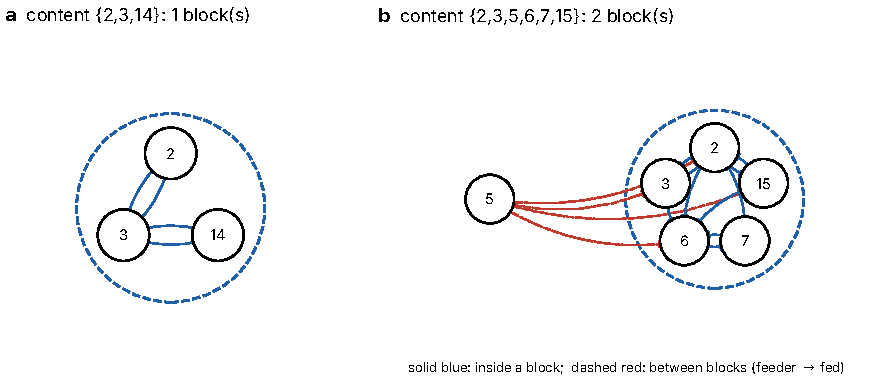
\includegraphics[width=\textwidth]{fig09_feeding_blocks}
\caption{\textbf{Feeding digraphs and blocks (exact).} Dashed blue circles are strongly connected blocks; solid blue arrows are feeding edges inside a block and dashed red arrows are feeding edges between blocks (feeder to fed). (a) $\{2,3,14\}$: one block ($3$ feeds $14$ and $14$ feeds $3$; $14$ does not feed $2$ or conversely). (b) $\{2,3,5,6,7,15\}$: the label $5$ is a block of its own feeding the block $\{2,3,6,7,15\}$. Theorems illustrated: \cref{thm:F2}, \cref{cor:F1}.}\label{fig:feeding}
\end{figure}
\noindent The figure above is \cref{fig:feeding}; its caption states the exactness of what is drawn.
\begin{figure}[tbp]\centering
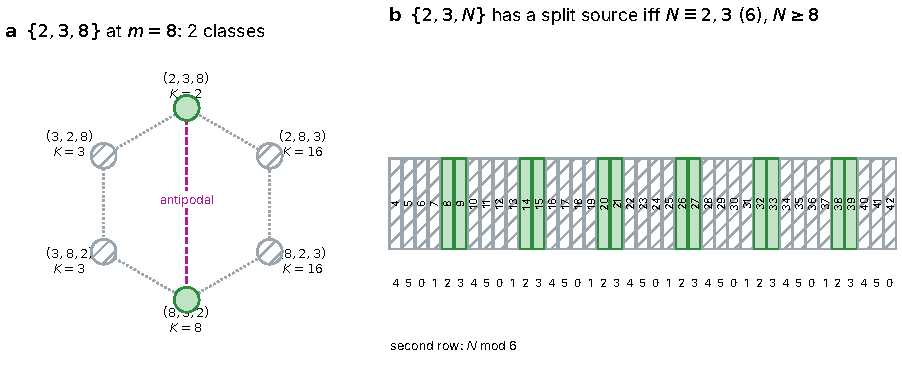
\includegraphics[width=\textwidth]{fig10_three_label_split}
\caption{\textbf{Three-label split and the antipodal orderings (exact; the strip is exact in the range shown).} (a) The hexagon of $\{2,3,8\}$ at $m=8$ with the threshold $K$ of each arrangement: only the antipodal pair $(2,3,8),(8,3,2)$ is admissible (two classes). (b) The integers $N=4,\dots,42$ with residues mod $6$: shaded cells are those for which $\{2,3,N\}$ has a split source, namely $N\equiv2,3\pmod 6$ with $N\ge8$. Theorems illustrated: \cref{thm:T3}, \cref{thm:23N}.}\label{fig:split}
\end{figure}
\noindent The figure above is \cref{fig:split}; its caption states the exactness of what is drawn.
\begin{example}[strongly connected, never split]\label{ex:sccnever}
The contents $\{2,4,15\}$, $\{2,5,9\}$ and $\{2,6,7\}$ have strongly connected feeding digraphs and $\nu\le1$ at every source in the lcm-closure of their thresholds. Strong connectivity of the feeding digraph is therefore necessary but not sufficient for a split.
\end{example}
\begin{proposition}[finite-exact: all three-label splits are antipodal]\label{prop:census3}
Among the $\binom{30}{3}=4060$ contents of three distinct labels in $\{1,\dots,30\}$, exactly $257$ have a strongly connected feeding digraph and exactly $127$ have a split source; each split content is strongly connected, so $130$ strongly connected contents never split. For each of the $4060$ contents and every source in the lcm-closure of its thresholds, the criterion of \cref{thm:T3} agrees with the direct class count (no violation). \stat{finite-exact}.
\end{proposition}
\prov{CW-0349}{THEOREMS\_V002:Census-FINITE-EXACT-results}{FINITE-EXACT}{FINITE}
